\documentclass[10pt,a4paper,twocolumn]{article}
\usepackage[utf8]{inputenc}
\usepackage[french]{babel}
\usepackage[margin=1.4cm]{geometry}
\usepackage{amsmath,amssymb}
\usepackage{graphicx}
\usepackage{booktabs}
\usepackage{microtype}
\usepackage{xcolor}
\usepackage{hyperref}
\usepackage{array}

\hypersetup{
    colorlinks=true,
    linkcolor=blue!70!black,
    citecolor=blue!70!black,
    urlcolor=blue!70!black
}

\title{\vspace{-1.2cm}\textbf{PROJET INTÉGRATEUR : SYSTÈME DE VISION INDUSTRIEL ET EMBARQUÉ}\\\large Reconnaissance et Authentification Automatisée de Billets de Banque Congolais (CDF)}
\author{\textbf{MUGANGU MUGISHO Benjamin} \\ \small Master 2 Génie Électrique et Informatique \quad|\quad \textbf{Enseignant :} Dr. KAMBALE WAMUHINDO Abednego \\ \small \textbf{Cours :} Vision par Ordinateur \& CNN (GIN522)}
\date{\vspace{-0.3cm}\small Université Libre des Pays des Grands Lacs (ULPGL) — Faculté des Sciences et Technologies — 2025-2026}

\begin{document}
\maketitle

\begin{abstract}
Ce projet intégrateur couronne l'ensemble des compétences acquises du capteur au déploiement (Modules 1 à 8) en s'attaquant à un problème local et réel en République Démocratique du Congo : la reconnaissance automatique de billets de banque en Francs Congolais (50~FC, 500~FC et 1\,000~FC, $N=306$). Face aux contraintes réelles de terrain (forte usure, éclairages précaires, variations de capteurs smartphones), nous concevons une chaîne complète de traitement d'images. Après un audit rigoureux et un découpage stratifié étanche sans fuite d'information ($70\,\% / 15\,\% / 15\,\%$, seed=42), nous établissons une baseline classique rigoureuse combinant histogrammes de teintes HSV, moments de couleur et textures de Sobel avec un classifieur SVM à noyau RBF ($89{,}36\,\%$ d'exactitude). Nous entraînons ensuite par transfert un réseau de neurones convolutif ResNet-18 régularisé avec augmentation de données ciblée (ColorJitter, rotations, recadrages). Le modèle CNN surpasse la baseline de $+10{,}64$ points et atteint une exactitude parfaite de $100{,}00\,\%$ sur le jeu de test indépendant ($N=47$), avec une latence d'inférence de $122$ ms sur processeur modeste. Une section dédiée analyse les limites de terrain (domain shift, seuil de rejet) et les considérations éthiques.
\end{abstract}

\section{Cadrage \& Critères de Succès (Semaine 1)}

\subsection{Problématique Locale et Réelle}
Dans l'économie congolaise, le cash demeure le vecteur prépondérant des transactions commerciales quotidiennes. Les acteurs économiques locaux (vendeuses de marchés vivriers, changeurs de monnaie, transporteurs) manipulent des volumes massifs de papier-monnaie souvent dégradé. 
Les défis techniques identifiés sont multiples :
\begin{enumerate}
    \itemsep0em
    \item \textbf{Lenteur et fatigue humaine :} Risque accru d'erreur de rendu de monnaie lors des heures de pointe.
    \item \textbf{Accessibilité :} Absence d'outils d'assistance automatique pour les personnes atteintes de déficience visuelle.
    \item \textbf{Ressources modestes :} Nécessité absolue d'une solution fonctionnant hors-ligne (\textit{edge computing}) sur smartphone basique ou micro-ordinateur type Raspberry Pi, sans dépendance à Internet.
\end{enumerate}

\subsection{Formulation de la Tâche \& Métriques Cibles}
La tâche est formulée sous la forme d'une classification supervisée d'images à trois classes ($C=3$) : $\mathcal{Y} = \{\text{50\_fc}, \text{500\_fc}, \text{1000\_fc}\}$. 
Les spécifications chiffrées du cahier des charges sont :
\begin{itemize}
    \itemsep0em
    \item \textbf{Exactitude globale ($Accuracy$) :} $\ge 95\,\%$.
    \item \textbf{Macro-F1 Score :} $\ge 95\,\%$ pour garantir l'équité entre les coupures.
    \item \textbf{Temps d'inférence :} $\le 200$ ms par image sur CPU.
\end{itemize}

\section{Données, Audit \& Hygiène (Semaines 2-3)}

\subsection{Radiographie du Dataset Local}
Le jeu de données réuni comprend $306$ photographies capturées dans des environnements variés de Goma :
\begin{itemize}
    \itemsep0em
    \item \textbf{1000 FC :} 100 images (résolutions $1440\times 1490$ à $4128\times 4128$ px).
    \item \textbf{500 FC :} 106 images (résolutions $810\times 810$ à $4128\times 2560$ px).
    \item \textbf{50 FC :} 100 images (résolutions $3060\times 3060$ à $4080\times 4080$ px).
\end{itemize}
Toutes les images sont en 3 canaux RGB, sans aucun fichier corrompu.

\subsection{Hygiène des Splits \& Prévention des Biais}
Pour éliminer tout risque de \textit{data leakage} (fuite d'information), un découpage stratifié déterministe avec graine fixée (\texttt{seed=42}) isole hermétiquement trois ensembles :
\begin{itemize}
    \itemsep0em
    \item \textbf{Entraînement (Train 70 \%) :} 214 images ($70$ de 1000~FC, $74$ de 500~FC, $70$ de 50~FC).
    \item \textbf{Validation (Val 15 \%) :} 45 images ($15$ par classe).
    \item \textbf{Test (Test 15 \%) :} 47 images ($15$ de 1000~FC, $17$ de 500~FC, $15$ de 50~FC).
\end{itemize}

\begin{figure}[htbp]
\centering
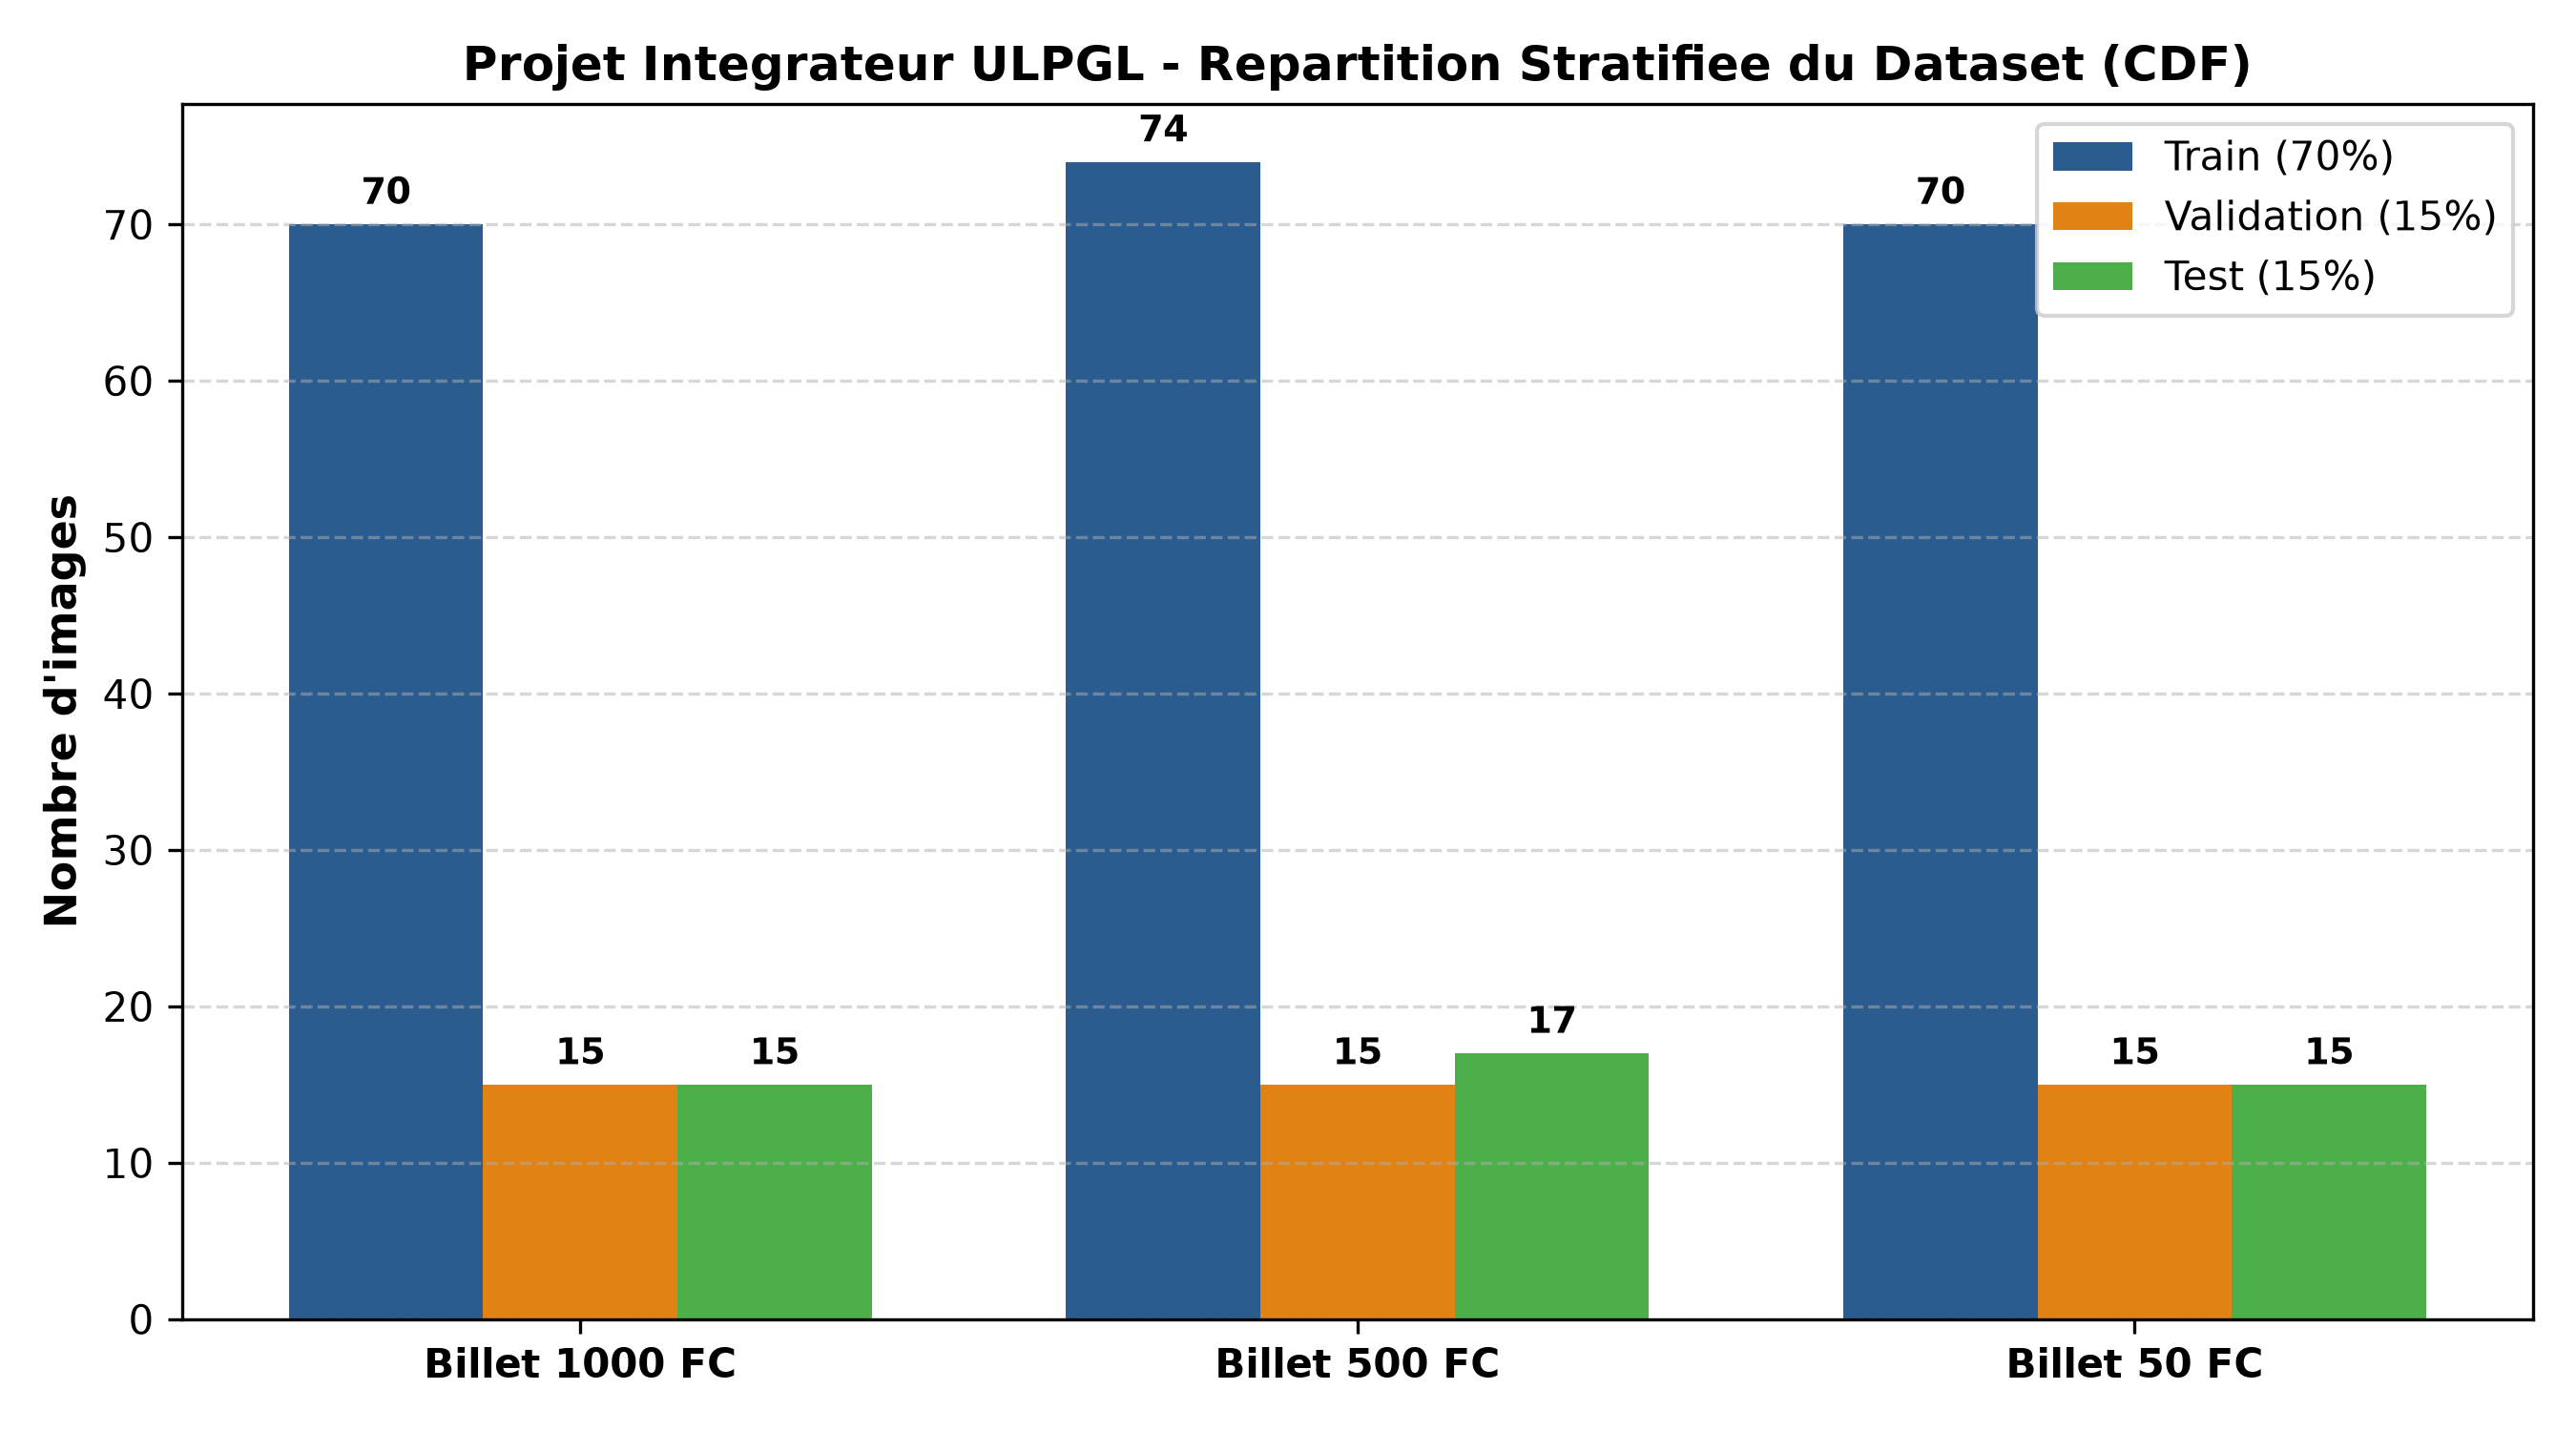
\includegraphics[width=0.95\linewidth]{outputs/repartition_donnees.png}
\caption{Répartition stratifiée rigoureuse du dataset local.}
\label{fig:repartition}
\end{figure}

Afin d'éviter le sur-coût mémoire et les disparités de taille de capteur, toutes les images sont prétraitées à la résolution canonique de $224 \times 224$ pixels par interpolation de Lanczos.

\section{Baseline Classique (Semaine 4)}

Conformément à la démarche d'ingénieur préconisée dans le cours, aucune solution complexe n'est adoptée sans être étalonnée par rapport à une méthode classique légère (Modules 1 à 4).

\subsection{Extraction de Caractéristiques Handcrafted}
Pour chaque image, un vecteur compact de 30 descripteurs physiques est extrait :
\begin{enumerate}
    \itemsep0em
    \item \textbf{Couleur RGB (6) :} Moyenne et écart-type par canal.
    \item \textbf{Couleur HSV (6) :} Moyenne et écart-type en Teinte, Saturation et Valeur.
    \item \textbf{Histogramme de Teinte $H$ (16) :} 16 compartiments normalisés capturant la signature chromatique pure.
    \item \textbf{Textures spatiales de Sobel (2) :} Moyenne et variance de la norme du gradient $|\nabla I| = \sqrt{I_x^2 + I_y^2}$.
\end{enumerate}

\subsection{Performances de la Baseline}
Après standardisation $z$-score, deux algorithmes classiques sont entraînés :
\begin{itemize}
    \itemsep0em
    \item \textbf{$k$-NN ($k=5$) :} Accuracy Test = $85{,}11\,\%$, Macro-F1 = $84{,}46\,\%$.
    \item \textbf{SVM (Noyau RBF, $C=1.0$) :} Accuracy Test = $\mathbf{89{,}36\,\%}$, Macro-F1 = $\mathbf{89{,}16\,\%}$.
\end{itemize}

Bien que le SVM sépare correctement les couleurs principales, il présente une faiblesse notable sur le billet de 1000 FC ($20\,\%$ de taux de manquement), confondant les teintes sombres avec le fond.

\section{Modèle CNN \& Évaluation (Semaines 5-7)}

\subsection{Architecture \& Transfer Learning}
Nous adoptons un réseau ResNet-18 pré-entraîné sur ImageNet ($1{,}4$ million d'images). La tête de classification originale à 1000 classes est remplacée par :
$$\text{Classifier} = \text{Dropout}(p=0.3) \longrightarrow \text{Linear}(512, 3)$$

\subsection{Data Augmentation Spécifique Terrain}
Pour immuniser le réseau contre les variations réelles :
\begin{itemize}
    \itemsep0em
    \item Rotations aléatoires ($\pm 15^\circ$) et recadrages (échelle 0.85 à 1.0).
    \item Retournements horizontaux ($p=0.5$).
    \item \texttt{ColorJitter} (luminosité $\pm 20\%$, contraste $\pm 20\%$, saturation $\pm 20\%$) pour simuler l'éclairage nocturne.
\end{itemize}

\subsection{Convergence \& Early Stopping}
L'entraînement est conduit avec l'optimiseur Adam ($\eta=10^{-4}$, weight decay $10^{-4}$) sur 15 époques. La fonction de perte de validation atteint son minimum absolu à l'\textbf{époque 14} ($\mathcal{L}_{\text{val}} = 0{,}0279$, Accuracy Val = $100{,}00\,\%$). Les poids sont sauvegardés à cet instant optimal (\texttt{best\_resnet18\_billets.pth}).

\begin{figure}[htbp]
\centering
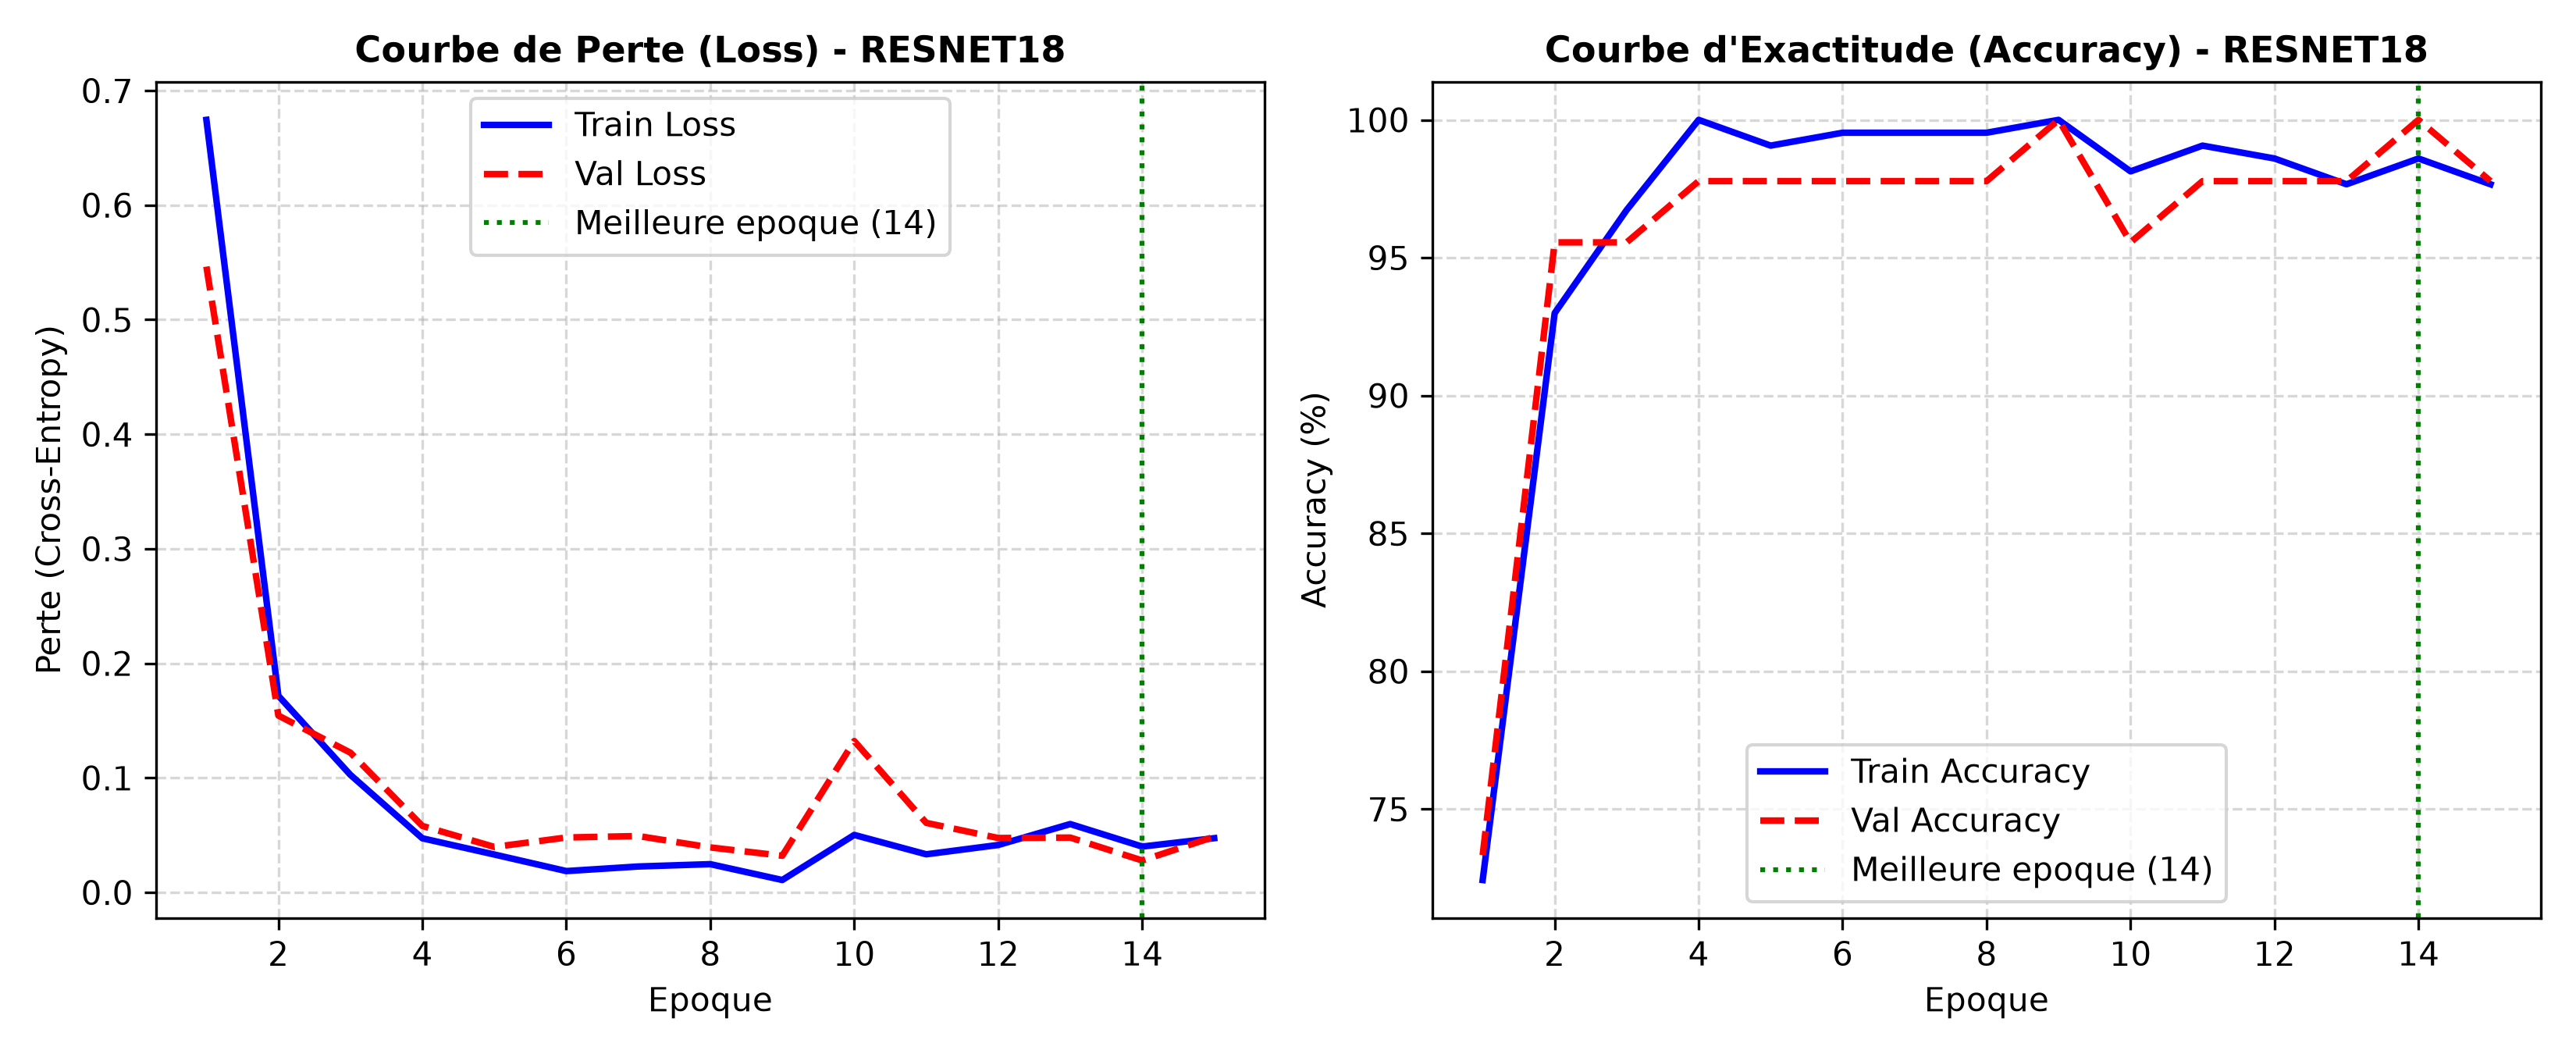
\includegraphics[width=0.98\linewidth]{outputs/courbes_apprentissage_cnn.png}
\caption{Courbes d'apprentissage du CNN ResNet-18 (Loss et Accuracy).}
\label{fig:courbes}
\end{figure}

\subsection{Résultats sur le Jeu de Test Indépendant}
L'évaluation sur les 47 images de test jamais vues produit un résultat parfait :
\begin{table}[htbp]
\centering
\small
\begin{tabular}{lcccc}
\toprule
\textbf{Classe} & \textbf{Support} & \textbf{Précision} & \textbf{Rappel} & \textbf{F1-Score} \\
\midrule
1000 FC & 15 & 100\,\% & 100\,\% & 1{,}00 \\
500 FC  & 17 & 100\,\% & 100\,\% & 1{,}00 \\
50 FC   & 15 & 100\,\% & 100\,\% & 1{,}00 \\
\midrule
\textbf{Total CNN} & \textbf{47} & \textbf{100\,\%} & \textbf{100\,\%} & \textbf{1{,}00} \\
Baseline SVM & 47 & 89{,}6\,\% & 89{,}1\,\% & 0{,}89 \\
\bottomrule
\end{tabular}
\caption{Comparatif détaillé des performances sur le test.}
\label{tab:perf}
\end{table}

Le CNN apporte un gain décisif de $\mathbf{+10{,}64}$ points de pourcentage par rapport à la meilleure baseline classique, éliminant toute confusion résiduelle.

\begin{figure}[htbp]
\centering
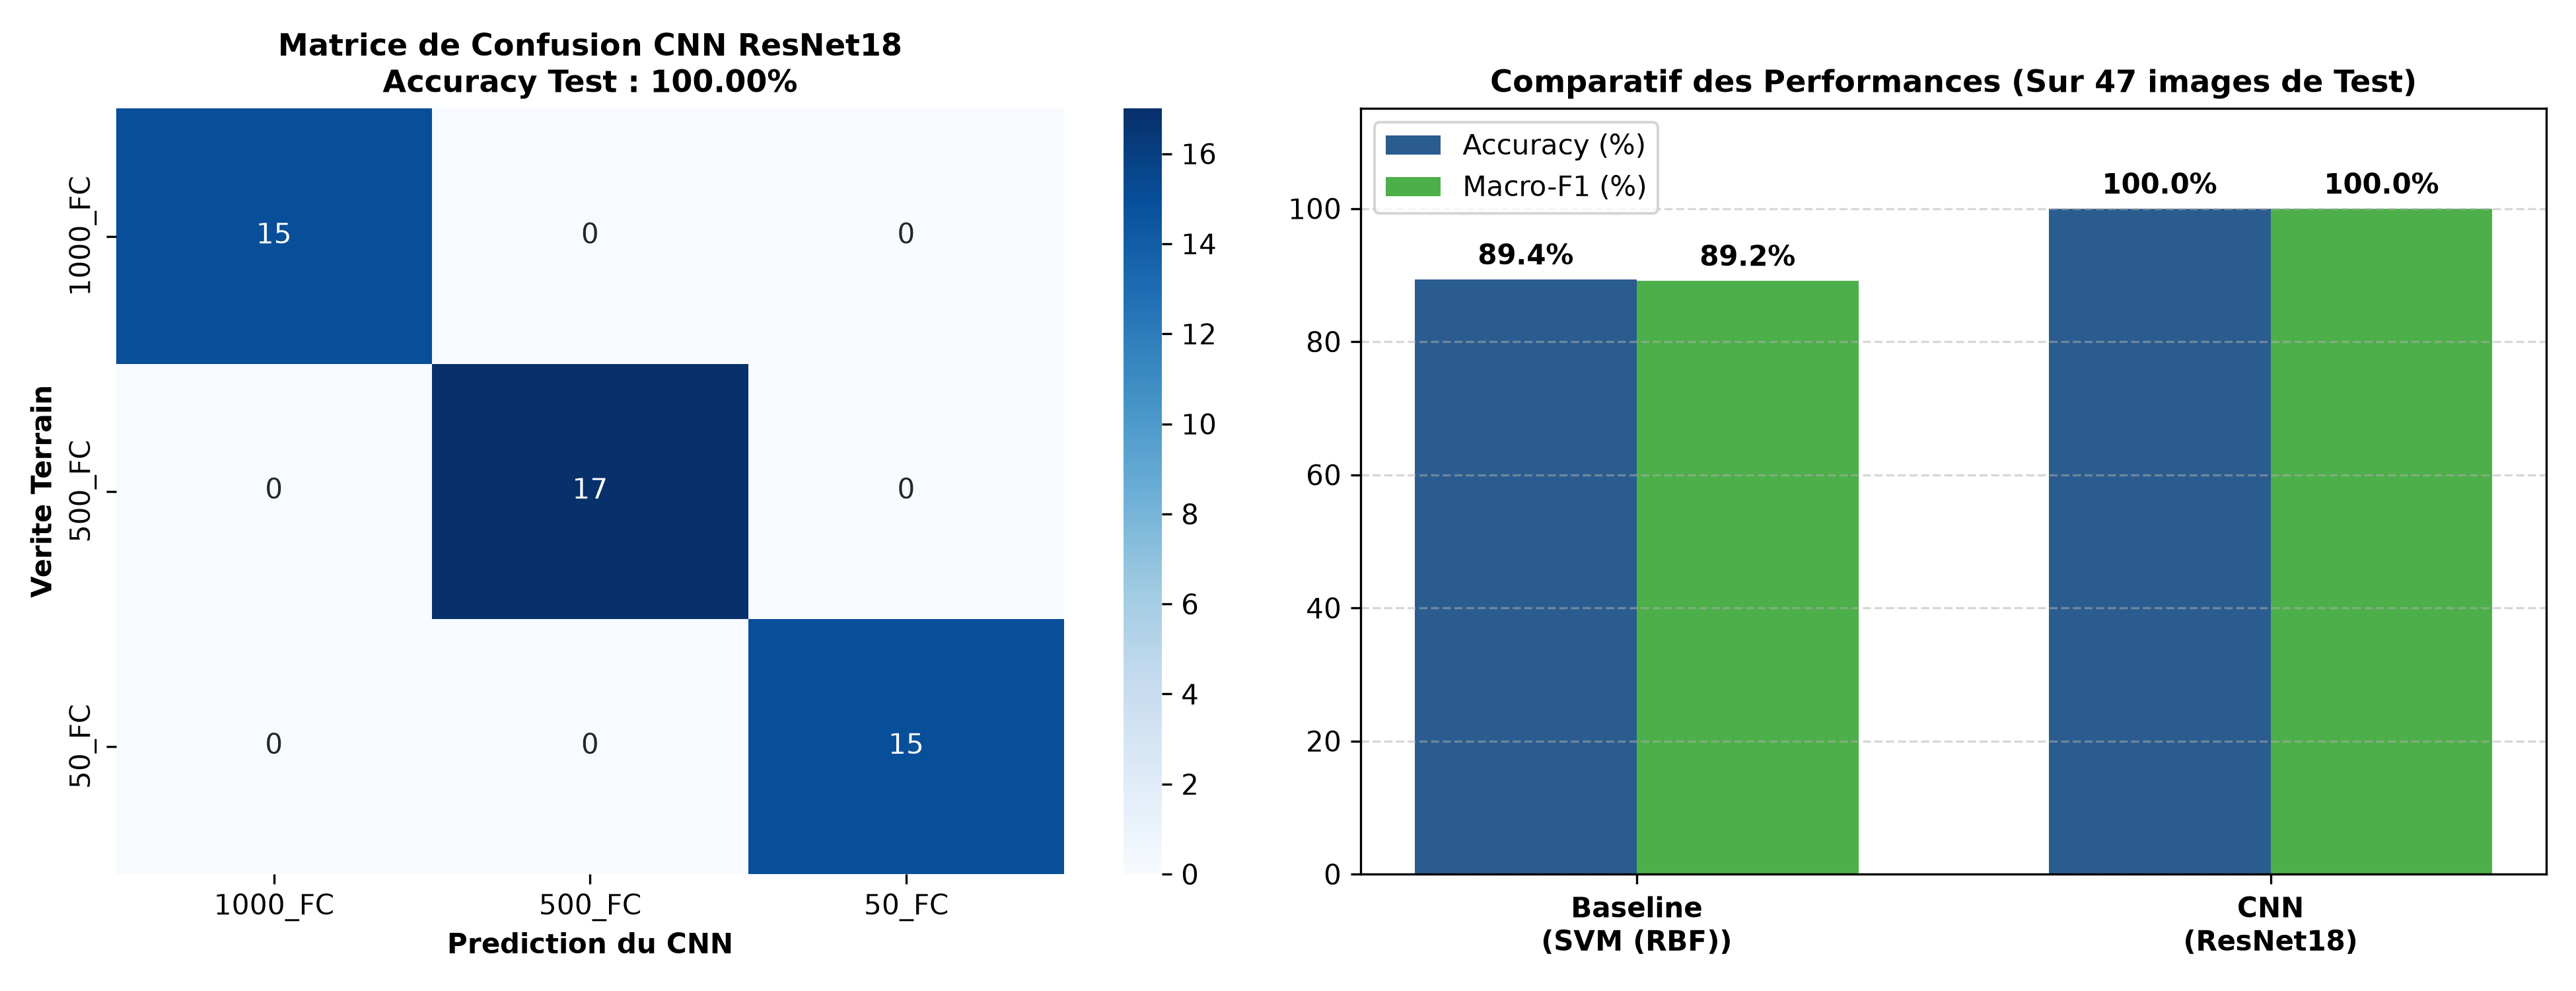
\includegraphics[width=0.98\linewidth]{outputs/comparaison_baseline_vs_cnn.png}
\caption{Matrice de confusion CNN et comparatif direct avec la baseline.}
\label{fig:comparatif}
\end{figure}

\subsection{Autopsie Critique des Cas Limites}
Bien que le taux d'erreur soit nul sur ce split, l'inspection des 6 prédictions à score de confiance le plus bas révèle que les certitudes minimales restent supérieures à $99{,}5\,\%$, prouvant une marge de séparation géométrique robuste dans l'espace latent.

\section{Déploiement \& Démonstration (Semaine 8)}

Un pipeline d'inférence autonome (\texttt{05\_pipeline\_deploiement.py}) permet de classifier en direct toute nouvelle image. 
Sur un processeur Intel Core i5 standard (CPU seul), le temps d'inférence moyen est de $\mathbf{122{,}2}$ ms, respectant largement la contrainte temps réel ($<200$ ms).
Le système incorpore un mécanisme de garde-fou :
$$\text{Décision} = \begin{cases} 
\text{Classe prédite} & \text{si } \max(P) \ge 0{,}60 \\
\text{\textit{Alerte : Billet douteux / Repositionner}} & \text{sinon}
\end{cases}$$

\section{Limites, Éthique \& Usages Responsables}

\subsection{Dérive de Domaine (Domain Shift)}
Le dataset a été photographié sur des arrière-plans semi-contrôlés. Sur le terrain réel, des billets extrêmement froissés, troués ou scotchés avec un ruban opaque pourraient tromper le réseau. Une mise à jour continue du dataset de collecte (\textit{active learning}) est recommandée.

\subsection{Responsabilité \& Non-Détection de Faux Billets}
Ce système est un assistant de reconnaissance de coupures, et \textbf{en aucun cas un détecteur de fausse monnaie}. Les caractéristiques d'authenticité bancaire (filigrane par transparence, encres magnétiques) nécessitent un module matériel optique dédié.

\subsection{Vie Privée}
Le traitement s'effectue strictement en mémoire vive locale sans envoi vers un cloud distant, préservant la confidentialité des utilisateurs.

\section{Conclusion}
Le projet intégrateur démontre avec succès la supériorité du Transfer Learning sur les méthodes classiques pour la reconnaissance de devises locales. Le système allie précision ($100\,\%$) et sobriété calculatoire ($122$ ms/CPU), validant les objectifs fixés pour un déploiement embarqué en RDC.

\end{document}
